%-*-latex-*-
% https://www.cs.cmu.edu/~ckingsf/bioinfo-lectures/quadtrees.pdf

\sectionthree{Quadtrees}
\begin{python0}
from solutions import *; clear()
\end{python0}

Quadtrees is a type trees used in
situations where you want to say something about closeness
of two things.
These (and many other related data structures) can be used
in games for collision detection
and they are also used in geospatial databases that is used
in geographic information systems.
I'm go focus only on quadtrees -- there are other
data structures for spatial indexing.

Suppose you have a collection of objects in a 2D space.
One common question to ask is when a pair (or more) of these
objects collided.
For simplicity, you can think of these objects are
rectangles (or circles, etc.)
The simplistic way for pairwise collision detection
is to perform a double for-loop on the objects
and check when they collde.
This has a runtime of $O(n^2)$.

Here's another way:
You think of a 2D area of your game (the whole window)
as a container of your game objects.
Suppose the window area is
$[0, 1000] \times [0, 1000]$
and there are 5 game objects:
\begin{center}
\begin{tikzpicture}

\draw (2.5, 2.5)
  node[draw, , , color=black,
       rounded corners=0cm, inner sep=0cm] {

\begin{minipage}[t][5cm]{5cm}
\mbox{}

\end{minipage}

};
\draw (-0.4, 4.6)
  node[draw=none, line width=0cm, , color=black,
       rounded corners=0cm, inner sep=0cm] {

\begin{minipage}[t][0.2cm]{0.1cm}
\mbox{}

\end{minipage}

};\draw (-0.4, 4.6) node[color=black] {$A$};
\draw (1.0, 1.0)
  node[fill=black,rounded corners=0cm,inner sep=0cm] {

\begin{minipage}[t][0.2cm]{0.2cm}
\mbox{}

\end{minipage}

};
\draw (1.0, 1.0)
  node[draw, , , color=black,
       rounded corners=0cm, inner sep=0cm] {

\begin{minipage}[t][0.2cm]{0.2cm}
\mbox{}

\end{minipage}

};
\draw (0.6, 1.0)
  node[draw=none, line width=0cm, , color=black,
       rounded corners=0cm, inner sep=0cm] {

\begin{minipage}[t][0.1cm]{0.1cm}
\mbox{}

\end{minipage}

};\draw (0.6, 1.0) node[color=black] {$p_{0}$};
\draw (4.5, 4.0)
  node[fill=black,rounded corners=0cm,inner sep=0cm] {

\begin{minipage}[t][0.2cm]{0.2cm}
\mbox{}

\end{minipage}

};
\draw (4.5, 4.0)
  node[draw, , , color=black,
       rounded corners=0cm, inner sep=0cm] {

\begin{minipage}[t][0.2cm]{0.2cm}
\mbox{}

\end{minipage}

};
\draw (4.1, 4.0)
  node[draw=none, line width=0cm, , color=black,
       rounded corners=0cm, inner sep=0cm] {

\begin{minipage}[t][0.1cm]{0.1cm}
\mbox{}

\end{minipage}

};\draw (4.1, 4.0) node[color=black] {$p_{1}$};
\draw (1.0, 4.0)
  node[fill=black,rounded corners=0cm,inner sep=0cm] {

\begin{minipage}[t][0.2cm]{0.2cm}
\mbox{}

\end{minipage}

};
\draw (1.0, 4.0)
  node[draw, , , color=black,
       rounded corners=0cm, inner sep=0cm] {

\begin{minipage}[t][0.2cm]{0.2cm}
\mbox{}

\end{minipage}

};
\draw (0.6, 4.0)
  node[draw=none, line width=0cm, , color=black,
       rounded corners=0cm, inner sep=0cm] {

\begin{minipage}[t][0.1cm]{0.1cm}
\mbox{}

\end{minipage}

};\draw (0.6, 4.0) node[color=black] {$p_{2}$};
\draw (2.0, 3.0)
  node[fill=black,rounded corners=0cm,inner sep=0cm] {

\begin{minipage}[t][0.2cm]{0.2cm}
\mbox{}

\end{minipage}

};
\draw (2.0, 3.0)
  node[draw, , , color=black,
       rounded corners=0cm, inner sep=0cm] {

\begin{minipage}[t][0.2cm]{0.2cm}
\mbox{}

\end{minipage}

};
\draw (1.6, 3.0)
  node[draw=none, line width=0cm, , color=black,
       rounded corners=0cm, inner sep=0cm] {

\begin{minipage}[t][0.1cm]{0.1cm}
\mbox{}

\end{minipage}

};\draw (1.6, 3.0) node[color=black] {$p_{3}$};
\draw (2.5, 1.5)
  node[fill=black,rounded corners=0cm,inner sep=0cm] {

\begin{minipage}[t][0.2cm]{0.2cm}
\mbox{}

\end{minipage}

};
\draw (2.5, 1.5)
  node[draw, , , color=black,
       rounded corners=0cm, inner sep=0cm] {

\begin{minipage}[t][0.2cm]{0.2cm}
\mbox{}

\end{minipage}

};
\draw (2.1, 1.5)
  node[draw=none, line width=0cm, , color=black,
       rounded corners=0cm, inner sep=0cm] {

\begin{minipage}[t][0.1cm]{0.1cm}
\mbox{}

\end{minipage}

};\draw (2.1, 1.5) node[color=black] {$p_{4}$};
\end{tikzpicture}

\end{center}


If there are too many game objects, say more than
$t = 4$, then you divide your
window into 4 equal size subwindows and distribute the game objects
into the appropriate subwindows of the game object is completely in a
subwindow.
If the game object is not completely in a subwindow, it stays in the
parent window.
\begin{center}
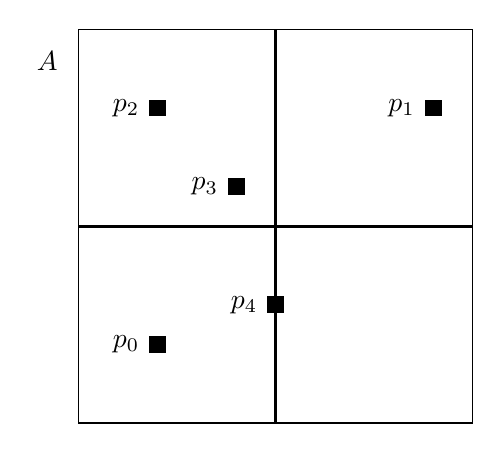
\begin{tikzpicture}

\draw (2.5, 2.5)
  node[draw, , , color=black,
       rounded corners=0cm, inner sep=0cm] {

\begin{minipage}[t][5cm]{5cm}
\mbox{}

\end{minipage}

};
\draw (-0.4, 4.6)
  node[draw=none, line width=0cm, , color=black,
       rounded corners=0cm, inner sep=0cm] {

\begin{minipage}[t][0.2cm]{0.1cm}
\mbox{}

\end{minipage}

};\draw (-0.4, 4.6) node[color=black] {$A$};
\draw (1.0, 1.0)
  node[fill=black,rounded corners=0cm,inner sep=0cm] {

\begin{minipage}[t][0.2cm]{0.2cm}
\mbox{}

\end{minipage}

};
\draw (1.0, 1.0)
  node[draw, , , color=black,
       rounded corners=0cm, inner sep=0cm] {

\begin{minipage}[t][0.2cm]{0.2cm}
\mbox{}

\end{minipage}

};
\draw (0.6, 1.0)
  node[draw=none, line width=0cm, , color=black,
       rounded corners=0cm, inner sep=0cm] {

\begin{minipage}[t][0.1cm]{0.1cm}
\mbox{}

\end{minipage}

};\draw (0.6, 1.0) node[color=black] {$p_{0}$};
\draw (4.5, 4.0)
  node[fill=black,rounded corners=0cm,inner sep=0cm] {

\begin{minipage}[t][0.2cm]{0.2cm}
\mbox{}

\end{minipage}

};
\draw (4.5, 4.0)
  node[draw, , , color=black,
       rounded corners=0cm, inner sep=0cm] {

\begin{minipage}[t][0.2cm]{0.2cm}
\mbox{}

\end{minipage}

};
\draw (4.1, 4.0)
  node[draw=none, line width=0cm, , color=black,
       rounded corners=0cm, inner sep=0cm] {

\begin{minipage}[t][0.1cm]{0.1cm}
\mbox{}

\end{minipage}

};\draw (4.1, 4.0) node[color=black] {$p_{1}$};
\draw (1.0, 4.0)
  node[fill=black,rounded corners=0cm,inner sep=0cm] {

\begin{minipage}[t][0.2cm]{0.2cm}
\mbox{}

\end{minipage}

};
\draw (1.0, 4.0)
  node[draw, , , color=black,
       rounded corners=0cm, inner sep=0cm] {

\begin{minipage}[t][0.2cm]{0.2cm}
\mbox{}

\end{minipage}

};
\draw (0.6, 4.0)
  node[draw=none, line width=0cm, , color=black,
       rounded corners=0cm, inner sep=0cm] {

\begin{minipage}[t][0.1cm]{0.1cm}
\mbox{}

\end{minipage}

};\draw (0.6, 4.0) node[color=black] {$p_{2}$};
\draw (2.0, 3.0)
  node[fill=black,rounded corners=0cm,inner sep=0cm] {

\begin{minipage}[t][0.2cm]{0.2cm}
\mbox{}

\end{minipage}

};
\draw (2.0, 3.0)
  node[draw, , , color=black,
       rounded corners=0cm, inner sep=0cm] {

\begin{minipage}[t][0.2cm]{0.2cm}
\mbox{}

\end{minipage}

};
\draw (1.6, 3.0)
  node[draw=none, line width=0cm, , color=black,
       rounded corners=0cm, inner sep=0cm] {

\begin{minipage}[t][0.1cm]{0.1cm}
\mbox{}

\end{minipage}

};\draw (1.6, 3.0) node[color=black] {$p_{3}$};
\draw (2.5, 1.5)
  node[fill=black,rounded corners=0cm,inner sep=0cm] {

\begin{minipage}[t][0.2cm]{0.2cm}
\mbox{}

\end{minipage}

};
\draw (2.5, 1.5)
  node[draw, , , color=black,
       rounded corners=0cm, inner sep=0cm] {

\begin{minipage}[t][0.2cm]{0.2cm}
\mbox{}

\end{minipage}

};
\draw (2.1, 1.5)
  node[draw=none, line width=0cm, , color=black,
       rounded corners=0cm, inner sep=0cm] {

\begin{minipage}[t][0.1cm]{0.1cm}
\mbox{}

\end{minipage}

};\draw (2.1, 1.5) node[color=black] {$p_{4}$};\draw[line width=0.04cm,black] (0,2.5) to  (5,2.5);
\draw[line width=0.04cm,black] (2.5,5) to  (2.5,0);
\end{tikzpicture}

\end{center}



Conceptually, as a tree, 
\begin{center}
\begin{tikzpicture}

\draw (2.5, 2.5)
  node[draw, , , color=black,
       rounded corners=0cm, inner sep=0cm] {

\begin{minipage}[t][5cm]{5cm}
\mbox{}

\end{minipage}

};
\draw (-0.4, 4.6)
  node[draw=none, line width=0cm, , color=black,
       rounded corners=0cm, inner sep=0cm] {

\begin{minipage}[t][0.2cm]{0.1cm}
\mbox{}

\end{minipage}

};\draw (-0.4, 4.6) node[color=black] {$A$};
\draw (2.5, 1.5)
  node[fill=black,rounded corners=0cm,inner sep=0cm] {

\begin{minipage}[t][0.2cm]{0.2cm}
\mbox{}

\end{minipage}

};
\draw (2.5, 1.5)
  node[draw, , , color=black,
       rounded corners=0cm, inner sep=0cm] {

\begin{minipage}[t][0.2cm]{0.2cm}
\mbox{}

\end{minipage}

};
\draw (2.1, 1.5)
  node[draw=none, line width=0cm, , color=black,
       rounded corners=0cm, inner sep=0cm] {

\begin{minipage}[t][0.1cm]{0.1cm}
\mbox{}

\end{minipage}

};\draw (2.1, 1.5) node[color=black] {$p_{4}$};\draw[line width=0.04cm,black] (0,2.5) to  (5,2.5);
\draw[line width=0.04cm,black] (2.5,5) to  (2.5,0);

\draw (-1.75, -2.75)
  node[draw, , , color=black,
       rounded corners=0cm, inner sep=0cm] {

\begin{minipage}[t][2.5cm]{2.5cm}
\mbox{}

\end{minipage}

};
\draw (-2.0, -2.5)
  node[fill=black,rounded corners=0cm,inner sep=0cm] {

\begin{minipage}[t][0.2cm]{0.2cm}
\mbox{}

\end{minipage}

};
\draw (-2.0, -2.5)
  node[draw, , , color=black,
       rounded corners=0cm, inner sep=0cm] {

\begin{minipage}[t][0.2cm]{0.2cm}
\mbox{}

\end{minipage}

};
\draw (-2.4, -2.5)
  node[draw=none, line width=0cm, , color=black,
       rounded corners=0cm, inner sep=0cm] {

\begin{minipage}[t][0.1cm]{0.1cm}
\mbox{}

\end{minipage}

};\draw (-2.4, -2.5) node[color=black] {$p_{2}$};
\draw (-1.0, -3.5)
  node[fill=black,rounded corners=0cm,inner sep=0cm] {

\begin{minipage}[t][0.2cm]{0.2cm}
\mbox{}

\end{minipage}

};
\draw (-1.0, -3.5)
  node[draw, , , color=black,
       rounded corners=0cm, inner sep=0cm] {

\begin{minipage}[t][0.2cm]{0.2cm}
\mbox{}

\end{minipage}

};
\draw (-1.4, -3.5)
  node[draw=none, line width=0cm, , color=black,
       rounded corners=0cm, inner sep=0cm] {

\begin{minipage}[t][0.1cm]{0.1cm}
\mbox{}

\end{minipage}

};\draw (-1.4, -3.5) node[color=black] {$p_{3}$};
\draw (1.25, -2.75)
  node[draw, , , color=black,
       rounded corners=0cm, inner sep=0cm] {

\begin{minipage}[t][2.5cm]{2.5cm}
\mbox{}

\end{minipage}

};
\draw (2.0, -2.5)
  node[fill=black,rounded corners=0cm,inner sep=0cm] {

\begin{minipage}[t][0.2cm]{0.2cm}
\mbox{}

\end{minipage}

};
\draw (2.0, -2.5)
  node[draw, , , color=black,
       rounded corners=0cm, inner sep=0cm] {

\begin{minipage}[t][0.2cm]{0.2cm}
\mbox{}

\end{minipage}

};
\draw (1.6, -2.5)
  node[draw=none, line width=0cm, , color=black,
       rounded corners=0cm, inner sep=0cm] {

\begin{minipage}[t][0.1cm]{0.1cm}
\mbox{}

\end{minipage}

};\draw (1.6, -2.5) node[color=black] {$p_{1}$};
\draw (4.25, -2.75)
  node[draw, , , color=black,
       rounded corners=0cm, inner sep=0cm] {

\begin{minipage}[t][2.5cm]{2.5cm}
\mbox{}

\end{minipage}

};
\draw (7.25, -2.75)
  node[draw, , , color=black,
       rounded corners=0cm, inner sep=0cm] {

\begin{minipage}[t][2.5cm]{2.5cm}
\mbox{}

\end{minipage}

};
\draw (7.0, -3.5)
  node[fill=black,rounded corners=0cm,inner sep=0cm] {

\begin{minipage}[t][0.2cm]{0.2cm}
\mbox{}

\end{minipage}

};
\draw (7.0, -3.5)
  node[draw, , , color=black,
       rounded corners=0cm, inner sep=0cm] {

\begin{minipage}[t][0.2cm]{0.2cm}
\mbox{}

\end{minipage}

};
\draw (6.6, -3.5)
  node[draw=none, line width=0cm, , color=black,
       rounded corners=0cm, inner sep=0cm] {

\begin{minipage}[t][0.1cm]{0.1cm}
\mbox{}

\end{minipage}

};\draw (6.6, -3.5) node[color=black] {$p_{0}$};\draw[line width=0.04cm,black] (2.29,-0.07) to  (-1.54,-1.43);
\draw[line width=0.04cm,black] (2.44,-0.07) to  (1.31,-1.43);
\draw[line width=0.04cm,black] (2.59,-0.07) to  (4.16,-1.43);
\draw[line width=0.04cm,black] (2.74,-0.07) to  (7.01,-1.43);
\end{tikzpicture}

\end{center}


Once $A$ has children, when a game object is placed in $A$,
if it is completely in one of the four subwindows, it is sent in  the
relevant subwindow for recursive insert.
If the game object intersects the boundary (look at the cross
in the window of $A$), then it stays in $A$.

Once a subwindow (again) has more than $t$ game objects.
you give this subwindow four children and repeat the distribution
of game objects into the children of the subwindow.

Once every game objects is distributed,
for the computation of collision detection,
you only need to check among the game objects in each leaf
subwindow, except that there might be game objects in the parent node.

$t$ is called the \defterm{threshold} of this quadtree.

To prevent building a tree that's has too many nodes,
you can also include a \defterm{maximum depth} in the nodes.
Say you want to limit the tree to maximum depth of 10.
Then once a node has reached a depth of 10, the node will not
expand into children nodes.
(Recall that the root has a depth of 0.)

Here are some obvious member variables each node of the tree should
have:
\begin{myenum}
  \li The geometry of the window: \verb!minx!, \verb!maxx!, \verb!miny!, \verb!maxy!
  \li Threshold (the $t$ from above)
  \li Depth of this node
  \li Maximum depth
  \li Array of pointers to game objects (it's probably best to use
  \verb!std::vector!, otherwise you would also need to have a
  size variable)
\end{myenum}
Note that the threshold and maximum depth are both applied throughout the
whole tree and therefore should probably be in the quad tree and not the quad
tree node.
Note that, of course, the quadtree must have access to the geometry/shape
of the game objects to know which subwindow a game object fits into.
It's convenient to have the following in a quad tree node:
\begin{myenum}
  \li A method to return the index of the child a game object should go into.
  \li A boolean member variable that tells you if the node has children.
\end{myenum}

A quad tree object has a pointer to the root node.
Besides that, you might also want the threshold and the maximum depth
in the quad tree.
Obviously methods includes a destructor, copy constructor, \verb!operator=!.
Besides that, of course you need to insert
(the pointer of) game objects into the tree.
Once all the (pointers of) game objects are placed in the quad tree,
you can start computing potential collisions groups.
This is done in two different ways:
\begin{itemize}
  \li Either get the quad tree to return
  a collection of \textit{all} colliding groups.
  The return type is \texttt{std::vector< std::vector< GameObject * > >}.
  (In general, a collision involves not just a pair of game objects.
  Depending on what you want to achieve in your game,
  in some cases, it is sufficient to compute \textit{pairs} of
  colliding game objects.)

  \li Or you might want to get 
  a collection of game objects colliding with \textit{a given
  game object}.
  The return type is \texttt{std::vector< GameObject * >}.
\end{itemize}

A quad tree has many uses besides game collision detection.
It is for instance used in computer graphics, image processing,
robotics, etc.
(which is natural since a quad tree is a spatial data structure).

[Note: Instead of rebuilding the whole quad tree for each
game loop, you can also update the quad tree. If the the space
is each cell is sufficiently large, the game object will
usually not change from one cell to another.
For this case, you would need to know if the (pointer of the) game object
has already been inserted into the quad tree or not.
If it's already in the quad tree, then it's an update operation.
However, the location of (pointer of) the game object in the quad tree
depends on the position of the game object during the last insert/update.
Therefore (and this is very important), each game object that is
updating its location in the quad tree
should contain the previous position and the current
The previous location allows you to find that game object in the
quad tree. Once the game object is found, if the current location
does not require the game object to move to a different quad tree node,
then nothing is done.
Otherwise it is deleted and then re-inserted into the
quad tree. Deleting of nodes in a quad tree is more complicated --
if the number of pointers in all children of node $n$
plus all the pointers in $n$ is $\leq$ threshold, then
all these pointers can go to $n$ and all the children nodes can be
deleted. However, it's possible that all these nodes might be re-created
again some time in the future.]

% We can also have a directory linked a game object pointer to a quad tree
% node pointer. Note that a game object can be later distributed into a
% child. So if $(g, n)$ is in this directory, g leads to a node n, but
% one might need to search in the subtree rooted at n in order to find g.

%\begin{ex}
%Recall that the distribution of data in a quad tree node
%to its children nodes is done for points not on the boundary
%of the subdivision -- the data on the boundary
%stays in the parent node.
%\end{ex}

\begin{ex}
  Based on what was described above, when computing
  collisions, do you need to check a node with
  it's grandparent?
\end{ex}
  
\begin{ex}
The quadtree is for subdividing a 2D space (a rectangular area).
The same idea can also be applied to an octtree where
a cube is divided into 8 equal sub-cubes in the obvious way.
Implement an octtree.
\end{ex}


\begin{comment}

The computation of checking pairs occurs in the leaves.
But some objects are some ancestor nodes too.
Therefore for the path from the root to the leaves must
collect up the game objects in the ancestor nodes.

So when traversing a quadtree, when you hit a leaf node,
you compute the collisions.
And what is the colllection of game objects you are
computing the collisions on?
Not just the game objects in the leaf node -- you
have to include all the game objects in
\textit{all} the ancestors of
that leaf node.

collisions:
    
    input:
        node
        ptrs = game object pointers from ancestors

    if self is leaf:
        return colliding pairs among (nodes.ptrs + ptrs)
    else:
        collision_groups = []
        collision_groups += collisions(node.child0, ptrs + node.ptrs)
        collision_groups += collisions(node.child0, ptrs + node.ptrs)
        collision_groups += collisions(node.child0, ptrs + node.ptrs)
        collision_groups += collisions(node.child0, ptrs + node.ptrs)
        return collision_groups
\end{comment}

\newpage
\section{kd trees}
